% Appendix C

% variables
\newcommand{\appdirc}{appendices/plots/appendixC}

\chapter{Geant4 simulation} % Main appendix title

\label{AppendixC} % For referencing this appendix elsewhere, use \ref{AppendixC}

\section{Simulation principle}
\label{appC:sec:simulation-principle}

The Geant4 software is a collection of tools and libraries to simulate particle interactions inside matter. The physics is described in terms of processes and models. The first is a description of a specific kind of physics interaction, a specific class handles when such interaction will occur along the track length. The model is the description of the details regarding a specific interactions, such as its specific kinematics. Geant4 allow more than one model to be used for a single proccesess, to allow the switch between different models following specific condition. An example is the switch between the Bertini cascade \cite{Heikkinen:2003sc} and the Fritiof (FTF) model at 25 \gev inside a specific physics list \cite{Uzhinsky:2013hea}. Monte Carlo methods are used to sample specific distributions and perform the simulation.

Particle transport is performed via a Stepping manager class that invokes actions processes, corresponding to physics interaction happening, and ``Trasportation processes'', which occur at the boundaries between different volumes. The expected length at which an interaction will occur is determined by polling all processes that are applicable to the track in the step computed. In practice, the true step length at each step is sample from the mean free path of the track inside the material where the steps occur and corrected by the \textit{step limitation} imposed at the beginning of the simulation. The mean free path of a process is defined as \cite{AGOSTINELLI2003250}:

\begin{equation}
  \label{eq:mfp-g4}
  \lambda(E) = \left( \sum_i [ n_i \cdot \sigma(Z_i,E)] \right)^{-1}
\end{equation}

Where $\sigma(Z_i,E)$ is the cross sections per atom of the process and the sum runs over all atom components inside the material. $n_i$ finally is the number of atoms of type i in the volume. The minimal step size is also limited as a compromise between speed of the simulation and accuracy of the results \cite{geant4-phys-guide}. The minimal dimension of the step is by default chosen to avoid change of cross-sections larger than $\sim$20\% due to energy loss, with some relaxation imposed for very low energy particles where this minimal step becomes too small.

In NA64, simulations are subdivided in different categories called ``examples'' inside the repository, each of them follows the same style and uses the same classes, but it is differentiated in the exact setup used, the presence or absence of Dark matter inside the model, and the precise output of it. Following the modular style of Geant4, C++ ``User'' classes are coded to extend the functionality of the basic Geant4 classes offered to control physics. We can divide this classes in multiple subgroup as function of their purpose in the simulation.

\begin{itemize}
\item \textbf{\textit{Geometry classes}}: These classes create the volumes used by the simulation. The class \textit{NA64DetectorConstruction} is the first class in hierarchical order, calling a set of subclasses to construct all different volumes of this setup. This approach has the advantage of simply removing part of the setup if needed by simply not calling the relevant class. Also it allows different detectors whose position or characteristic depends from other detectors to communicate those parameters via the class \textit{ParameterDBase} and throw an error if the relevant class was not yet called.
\item \textbf{\textit{Physics classes}}: These classes initialize the relevant physic to simulate and apply biases to specific cross-section if required by the study. The main classes of this type are \textit{NA64RunAction} and \textit{NA64RunActionWithA}. The first one initializes additional interactions not included in the modular physics list \textit{FTFP\_BERT}, namely the Synchrotron Radiation via \textit{G4SynchrotronRadiation} and dimuon conversion via \textit{G4GammaConversionToMuons}. A bias to these two interaction is optionally added by calling the method \it{SetCrossSecFactor} that set a multiplier to the total cross-section computed by the underlying model.
\item \textbf{\textit{Output classes}}: These classes are used to extract relevant information produced in the MC-simulation and write them on an output file after proper modification are performed. To date only the class \textit{NA64SD.cc} is part of this group. Methods of this class are called each time a ``sensitive detector'' is crossed by a track. Sensitive detectors are defined internally to each geometry class and corresponds to the active area of the detectors used in NA64.
\end{itemize}


Between all of them, the class \textit{NA64DetectorConstruction} act as a messenger between all classes, handling the transmission of relevant variables if they are needed.

%\section{The physics list}
%\label{appC:sec:physics-list}

\section{Interaction biasing}
\label{appC:sec:physics-list}

In this section a small description of the concept behind event biasing is provided and applied to the biasing of electronuclear and photonuclear interaction, which is the main background predicted for the invisible mode of NA64. What follows is an extract of the master work of one of the master student that worked together with me at these estimates \cite{pdegen-thesis}.

Due to the small cross sections of electronuclear and photonuclear interactions, it is not computationally feasible to simulate enough events for a proper analysis with statistics comparable to the data. Hence the probability of rare events has to be artificially increased using event biasing (variance reduction) techniques. The basic idea behind cross section biasing, also called \textit{Physics Process Occurrence Biasing} in Geant4 \cite{G4bias}, is to replace the analog (natural) interaction law by a biased one and then compute statistical weights that can be used to ``de-bias'' the results and get the correct distributions of the analog quantities. This stands in contrast to non-physics-based biasing techniques such as splitting and killing, which introduce or remove particles without changing the underlying physics process.

It must be noted that many official biasing techniques in Geant4 are state of the art features that are still under development at time of writing. In particular, biasing of cross sections for charged particles is not yet officially supported by Geant4. The issue is how much the cross section varies from the beginning of the step (the basic unit along which Geant4 propagates its particles) to the point of interaction. The currently implemented internal biasing method assumes that there is no change of cross section, which technically makes this method only applicable to neutral particles. However, since electronuclear interactions have a particularly small cross section, it is worth investigating whether this change is negligible and the neutral case can be applied.

It should also be mentioned that for simplicity the pre-existing software simulation package at NA64 features a custom biasing method that does not use any statistical weights for de-biasing. Instead, this method directly accesses the Geant4 source files \verb|G4ElectroNuclearCrossSection.cc| and \verb|G4PhotoNuclearCrossSection.cc| and multiplies the respective cross sections by a constant biasing factor if certain conditions are met. Since only upstream interactions were of interest for the estimation of the hadronic background, the following two biasing conditions were imposed:

\begin{itemize}
    \item the incident particle must have a kinetic energy > \SI{90}{\giga\electronvolt},
    \item the target nucleus must have an atomic number Z < 80,
\end{itemize}

\noindent which was deemed a convenient way to prevent the Pb layers in the ECAL target from being biased as well. 

Before investigating the de-biasing method more thoroughly, it is instructive to discuss the choice of the biasing factor $k$. The analog interaction probability $P_{I,a}(d)$ of a particle traversing a target as a function of the penetration depth $d$ is given by the integral of the exponential distribution
%
\begin{equation}
    P_{I,a}(d) = \int_0^d n\sigma_a e^{-n\sigma_a s}ds,
    \label{eq:analog_pdf}
\end{equation}
%
where $n$ is the number density of the target and $\sigma_a$ is the analog cross section. This expression assumes that the cross section is independent of $d$, which is only valid for neutral particles traversing a homogeneous volume of a single material. The homogeneity condition is always satisfied in Geant4 since the fundamental, discrete length unit along which particles are propagated never crosses the boundary between different volumes. Next we bias the cross section as $\sigma_b = k\sigma_a$ and introduce the mean free paths $\lambda_a = 1 / n \sigma_a$ and $\lambda_b = 1 / n \sigma_b$. We can now calculate the total number of biased interactions $N_{int}$ for a given number of incident particles $N$ traversing a target of thickness $d$ as
%
\begin{equation} \label{eq:n_int}
\begin{split}   
    N_{int} &= N \times P_{I,b}(d)\\
    &= N \times \int_0^d \frac{1}{\lambda_b}b e^{-s/\lambda_b} ds\\
    &= N \times (1-e^{-d/\lambda_b})\\
    &\simeq N \times (1-(1-d/\lambda_b))\\
    &= N \times d/\lambda_b\\
    &= Nk \times d/\lambda_a\\
    &\simeq Nk \times P_{I,a}(d),
\end{split}
\end{equation}
%
from which we can see that, in the case of thin targets with $d / \lambda_a \ll 1$, biasing the cross section yields an equivalent number of interactions as the unbiased process with an increase in the number of incident particles by a factor of $k$. The expansion $\mathrm{exp}(-d\lambda_b) \simeq 1- d/\lambda_b$ also gives us the condition on the biasing factor:
%
\begin{equation} \label{eq:bias_estimate}
\begin{split}   
d/\lambda_b &\ll 1\\
\rightarrow k &\ll \lambda_a/d.
\end{split}   
\end{equation}
%
In other words, the biasing factor has an upper threshold given by the inverse target thickness in units of the mean free path. On the other hand, choosing too large a biasing factor such that the biased mean free path is considerably smaller than the target thickness runs danger of beam depletion (premature absorption of the incident particle). That said, this threshold is not be understood as a hard limit, but rather as a general reference point from which a further study of the biasing factor should be embarked on. We will shortly see that in the NA64 2018 invisible mode the MM detectors are responsible for most of the upstream electronuclear interactions. Using an older estimate of their nuclear interaction length thickness of $d_{\lambda} = 1.9 \times 10^{-3}$, we thus find $k \lesssim 500$, though the actual value is likely smaller.

When using biased simulations, one has to keep in mind that analog quantities related to the biased ones are necessarily also distorted. For example, in cross section (occurrence) biasing, we only want to increase the number of rare events, but since the cross section is inversely related to the mean free path, the latter will be unphysically decreased by a factor of $k$. As mentioned in the beginning of this section, the solution to this is to compute statistical weights that can be used to de-bias the analog quantities \cite{G4bias,Mendenhall_2012}. It is thus instructive to compare the NA64 custom biasing method (represented by the unweighted case) and the internal Geant4 biasing method.

We start by defining the weight, which in general is a function of the random variable under consideration and is given by the ratio of analog and biased probability densities
%
\begin{equation} \label{eq:weight}
w(x) = \frac{p_a(x)}{p_b(x)},
\end{equation}
%
provided that $p_b(x)$ is non-zero for all $x$ where $p_a(x)$ is non-zero. In the case of occurrence biasing, $x$ is given by the interaction distance of the current step and $p(x)$ by the exponential law. Additionally, there are actually two weights that have to be taken into account:
%
\begin{itemize}
    \item When a particle travels from 0 to $d$ without interaction, it has a different probability to do so in the biased and analog schemes. Defining the probability of non-interaction as $P_{NI} = 1 - P_{I}$, the resulting weight is given by
    %
    \begin{equation} \label{eq:weight_NI}
    \begin{split}
    w_{NI}(d) &= P_{NI,a}(d)/P_{NI,b}(d)\\
    &=e^{-n\sigma_a d}/e^{-n\sigma_b d}\\
    &= e^{n\sigma_a d(k-1)}.
    \end{split}
    \end{equation}
    %
    If there are several biased process at play, each with their own dedicated interaction law, the resulting overall weight is given by the product of the individual weights. Here one can also see that the exponential will quickly become very large unless condition \ref{eq:bias_estimate} is satisfied.
    \item Similarly, if the particle makes an interaction in the next segment $ds$ with probability $P_I = p_I ds$, the weight is given by the ratio of the biased and analog probabilities
    %
    \begin{equation} \label{eq:weight_I}
    \begin{split}
    w_{I} &= P_{I,a}/P_{I,b}\\
    &=(1-e^{-n\sigma_a ds})/(1-e^{-n\sigma_b ds})\\
    &\simeq \sigma_a / \sigma_b\\
    &= 1/k,
    \end{split}
    \end{equation}
    %
    where in this case we have expanded the exponential due to $ds \ll d$. Here, in the case of multi-process biasing, the relevant weight is given solely by the weight of the actual process that is taking place. It should also be noted that in general $\sigma_b$ may depend on $d$ even in homogeneous materials, for example in forced collision biasing where an interaction is forced to occur in the segment $[0,L]$ (corresponding to a truncated exponential law). However, this is not the case for pure cross section biasing as presented in this study.
\end{itemize}
%
In the context of a concrete implementation in Geant4, $d$ represents the step along which particles are propagated. The non-interaction weight is calculated for every step in a biased detector volume. The biased cross section for discrete processes is computed at the post-step point and in case of an interaction multiplied with the non-interaction weight of the step. In this manner the weights are evolved multiplicatively for each step of a given particle. The weights also get passed along as starting weights to any daughter particles created. The user can access the current weight of the track at any point via the method \verb|GetWeight()|, which can then be used to reweigh desired physical quantities accessed through a custom scoring method (e.g. via the \verb|G4UserSteppingAction| or \verb|G4SensitiveVolume|). This reweighting is typically done by applying the weight to the fill function of a histogramming tool such as ROOT \cite{root}.

\begin{figure}[htb]
  \centering
  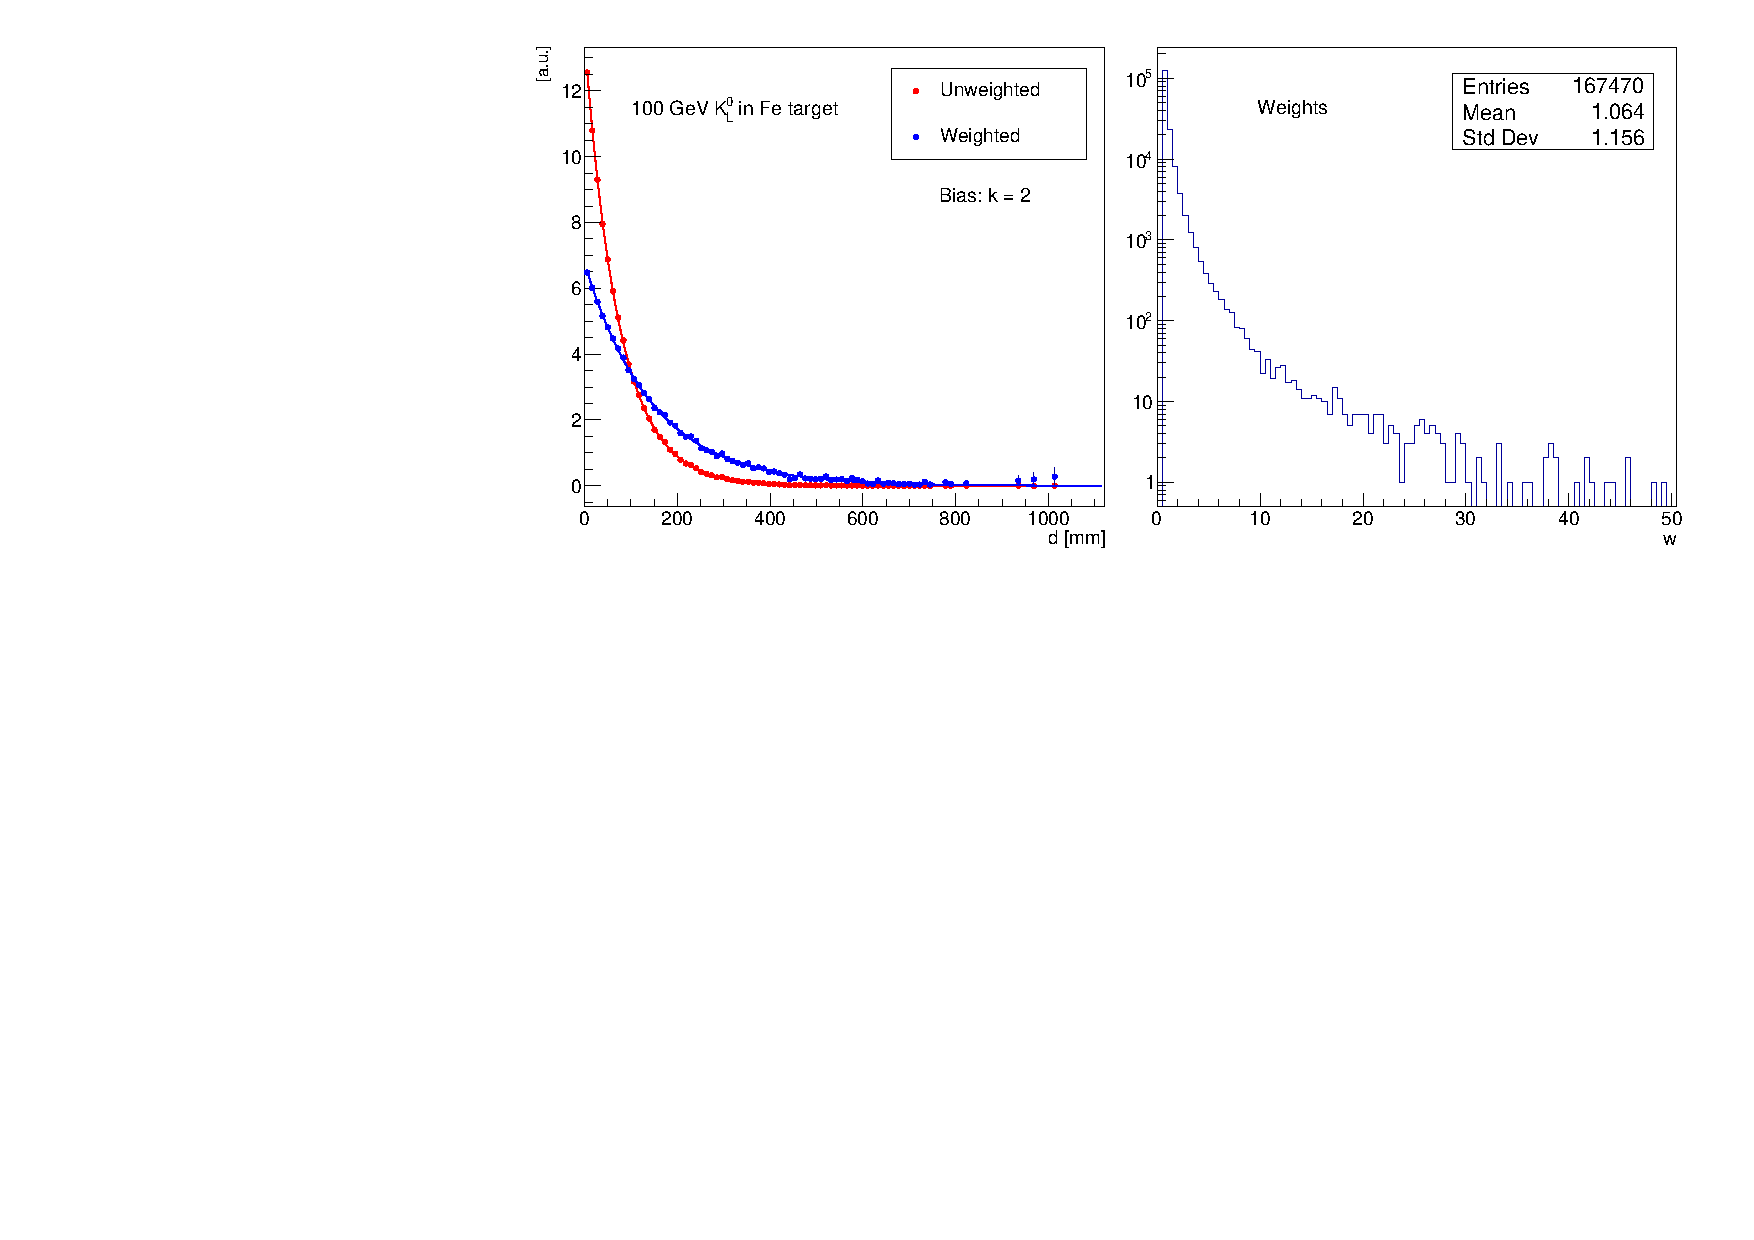
\includegraphics[width=0.8\linewidth]{\appdirc/klong.pdf}
  \caption[Distribution of interaction lengths of $\mathrm{K^0_L}$ inelastic scattering.] {Distribution of interaction lengths of 100~GeV~$\mathrm{K^0_L}$ inelastic scattering inside a thick Fe target for a biasing factor $k=2$. The resulting mean free paths can be found in \ref{res:Tab:meanfreepaths}.}
  \label{res:fig:klong}
\end{figure}

As an example, \ref{res:fig:klong} shows a simulation of longitudinal vertex positions of the inelastic scattering of 100~GeV~$\mathrm{K^0_L}$ inside a thick iron target for a biasing factor of $k$~=~2. The mean free path can be extracted by fitting an exponential to the resulting distribution and taking the inverse of the fit parameter specifying the slope of the exponential. Being neutral particles, Geant4 should be able to calculate the corresponding weights correctly. Indeed, as can be seen from \ref{res:Tab:meanfreepaths}, the ratio between the weighted and unweighted mean free paths corresponds very closely to the biasing factor. The same result was also found for $\pi+$ inelastic scattering, despite being a charged particle. It would be interesting to see at which point the de-biasing breaks down for charged particles, however, large biasing factors cannot be chosen for processes in thick targets that have a naturally large rate of occurrence because clearly condition \ref{eq:bias_estimate} is not satisfied. Regardless of whether the particle is charged or not, choosing a large biasing factor would cause most interactions to occur right at the beginning of the target, degrading the statistical quality of points deeper inside. Finally, the last column of \ref{res:Tab:meanfreepaths} shows the interaction lengths of the electronuclear interaction. One can see that for increasing biasing factors the weighted interaction lengths increase in size relative to the unbiased interaction length.


\begin{table}[htbp]
	\centering
	\caption[Simulated interactions lengths of various hadronic processes in a thick Fe target for different biasing factors.]{Simulated interactions lengths of various hadronic processes in a thick Fe target for different biasing factors. For comparison, the PDG value for the nuclear interaction length of Fe is \SI{16.77}{\centi\metre} and the pion interaction length is \SI{20.42}{\centi\metre} \cite{nist-database}.}
	\begin{tabular}{|r@{}l|c|c|c|}
		\toprule
		\multicolumn{2}{c|}{Bias} & $\mathrm{K^0_L}$ inelastic [cm]& $\pi^+$ inelastic [cm]& Electronuclear [cm]\\
		\midrule
		k&=1 & 14.63(7) & 19.75(3)  & 750(30)\\
		k&=2 weighted & 14.67(7) & 19.69(8)& 777(19)\\
		k&=2 unweighted & 7.34(2) & 9.872(19) & 456(7)\\
		k&=10 weighted & 14.4(5) & 19.9(4) & 840(30) \\
		k&=10 unweighted & 1.475(4) & 1.980(4) & 107.1(5)\\
		k&=50 weighted & - & - & 880(90) \\
		k&=50 unweighted & - & - & 219.6(6)\\
		k&=200 weighted & - & - & 920(240) \\
		k&=200 unweighted & - & - & 5.513(9)\\
		\bottomrule
	\end{tabular}
	\label{res:Tab:meanfreepaths}
\end{table}

Since the full implementation of an advanced event biasing method that correctly implements the weights for electronuclear interactions was beyond the scope of this thesis, the electronuclear and photonuclear cross sections were both biased by a factor of 200 using the existing NA64 biasing method. To make sure this method leads to sensible results, a comparison of biased and unbiased $R$ distributions is given in \ref{res:fig:biascomp}. In order to do a meaningful comparison, only events that have at least one electronuclear interaction occurring anywhere before the target are taken into account. Put differently, instead of using statistical weights to compensate the biased distribution for comparison with the full unbiased sample, the unweighted biased distribution is compared to only a subset of the unbiased sample which reflects the rare process that we want to bias in the first place. The distributions are clearly in decent agreement, giving a preliminary justification for the use of biased simulations for the comparison of simulated $R$ values with the data.
%
\begin{figure}[htb]
    \centering
    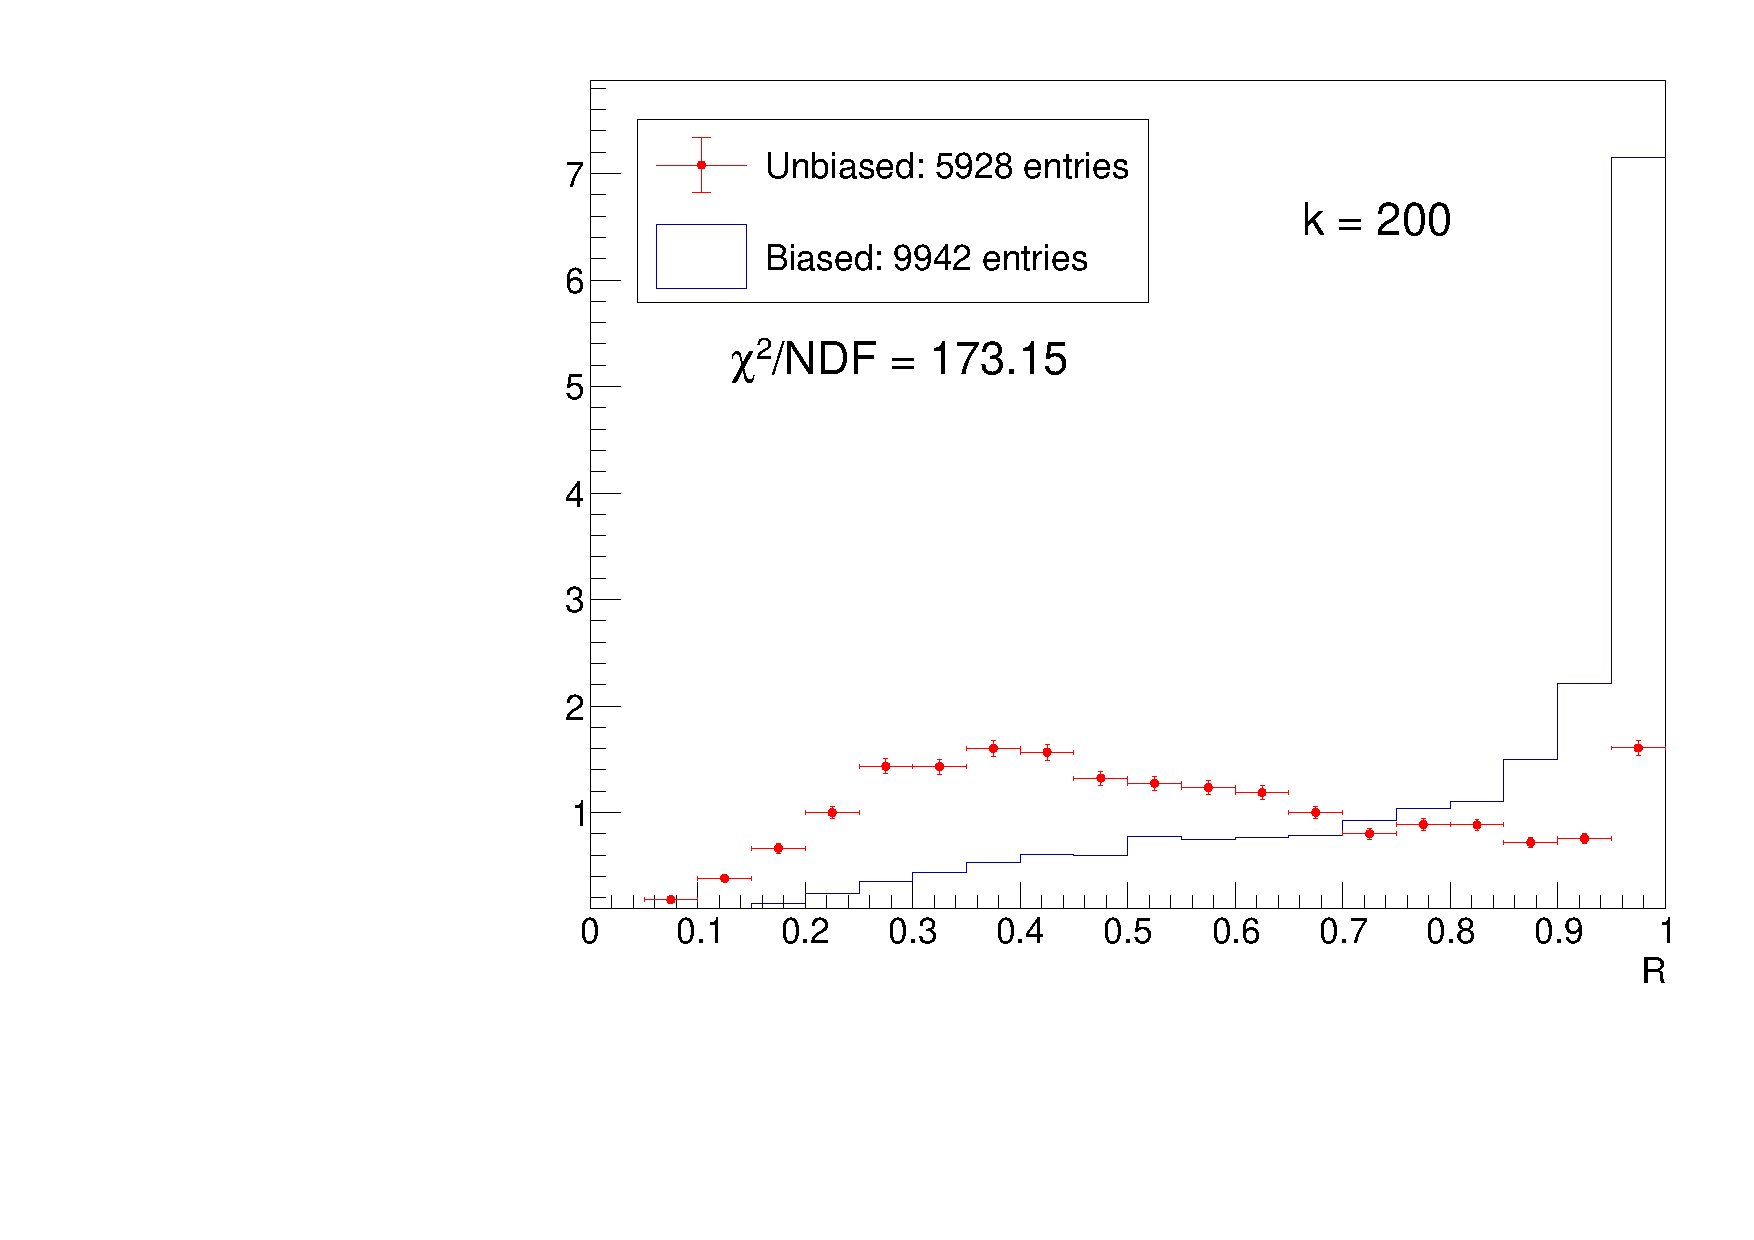
\includegraphics[width=0.45\textwidth]{\appdirc/pp48-comparison-bias-unbias-full2.pdf}
    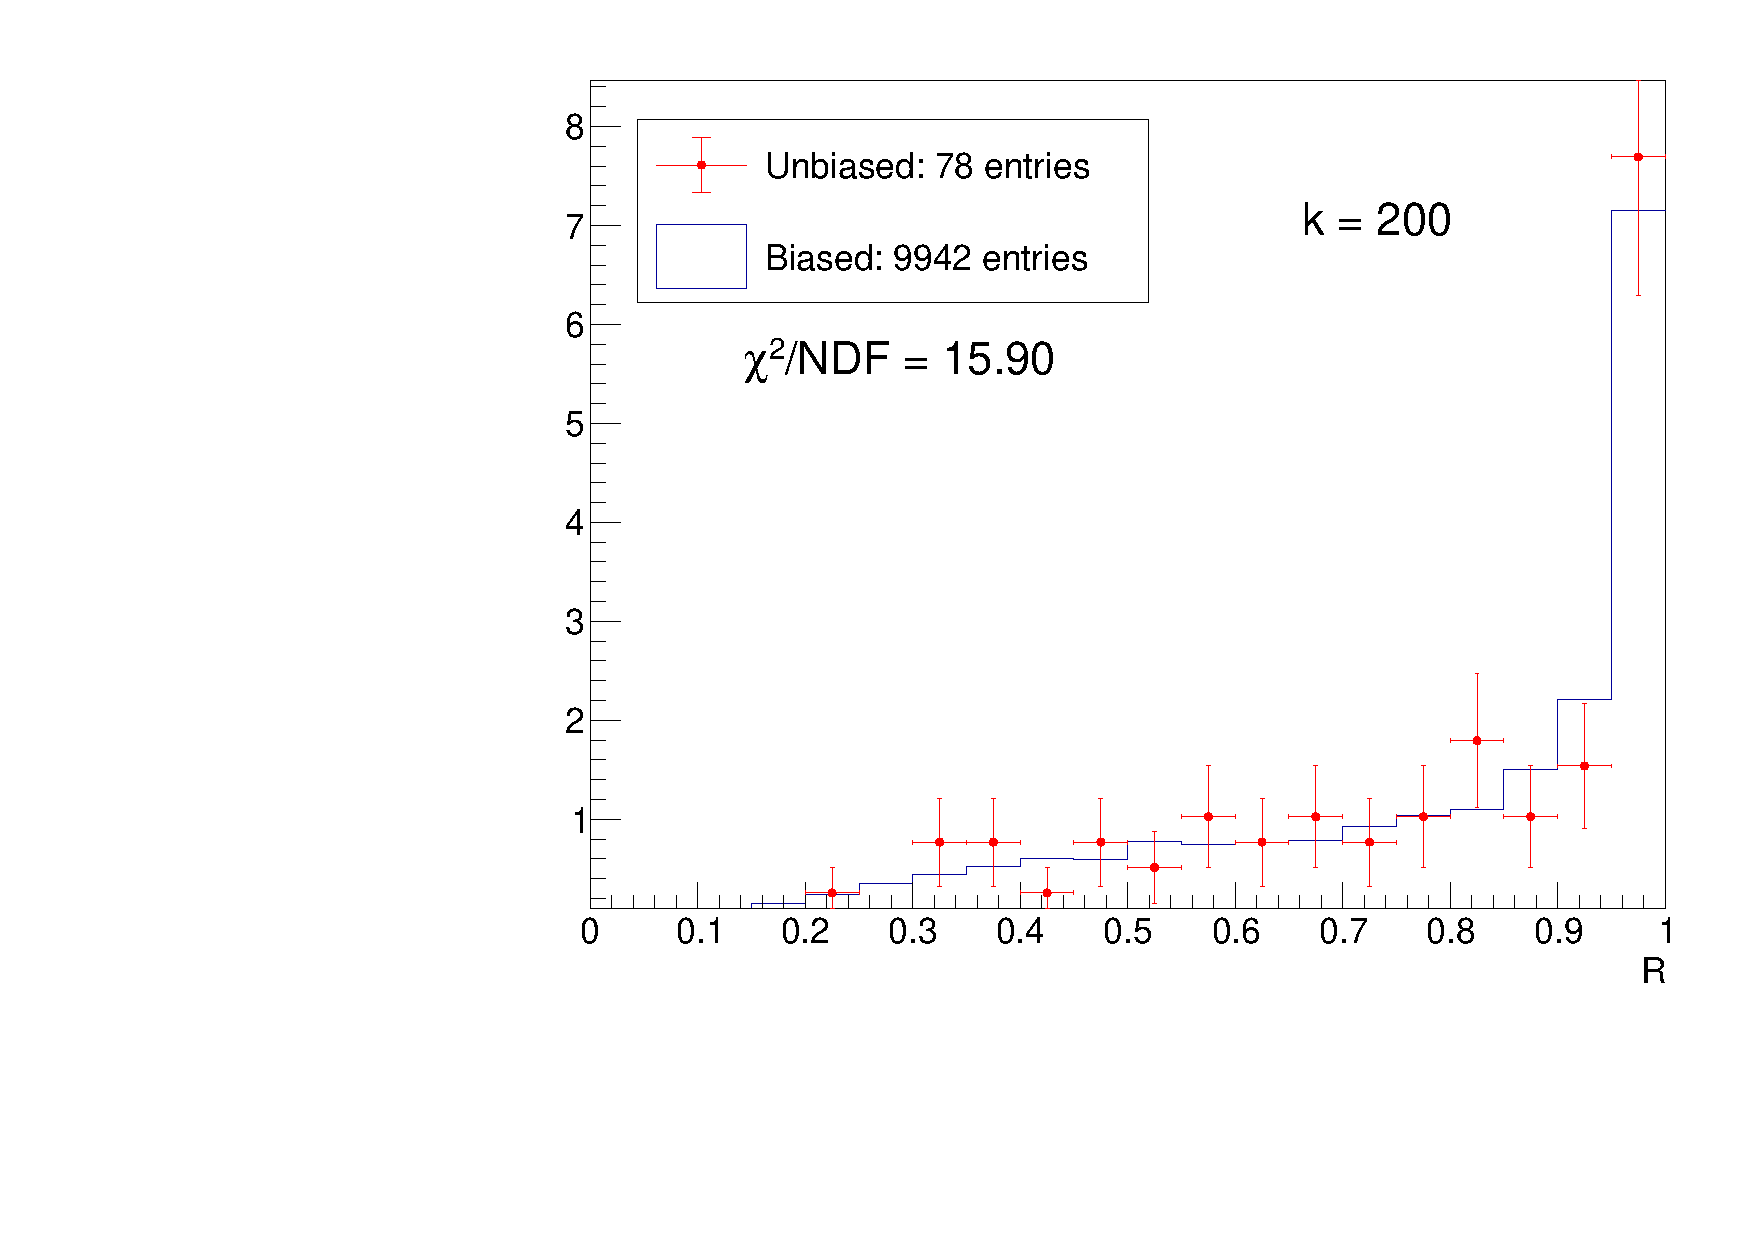
\includegraphics[width=0.45\textwidth]{\appdirc/pp48-comparison-bias-unbias2.pdf}
    \caption[Comparison of biased and unbiased $R$ distributions.]{Comparison of biased and unbiased normalized $R$ distributions before (left panel) and after (right panel) applying a cut that requires at least one electronuclear interaction to occur upstream of the target. Bremsstrahlung and dimuon events were removed using the cuts described in \ref{res:Tab:mccuts}.}
  \label{res:fig:biascomp}
\end{figure}

As mentioned earlier, only the upstream part of the detector was biased, which was achieved by using conditions on the incident particle kinetic energy and atomic number of the target nucleus. This can be seen explicitly in \ref{res:fig:enz},
%
\begin{figure}[htb]
  \centering
  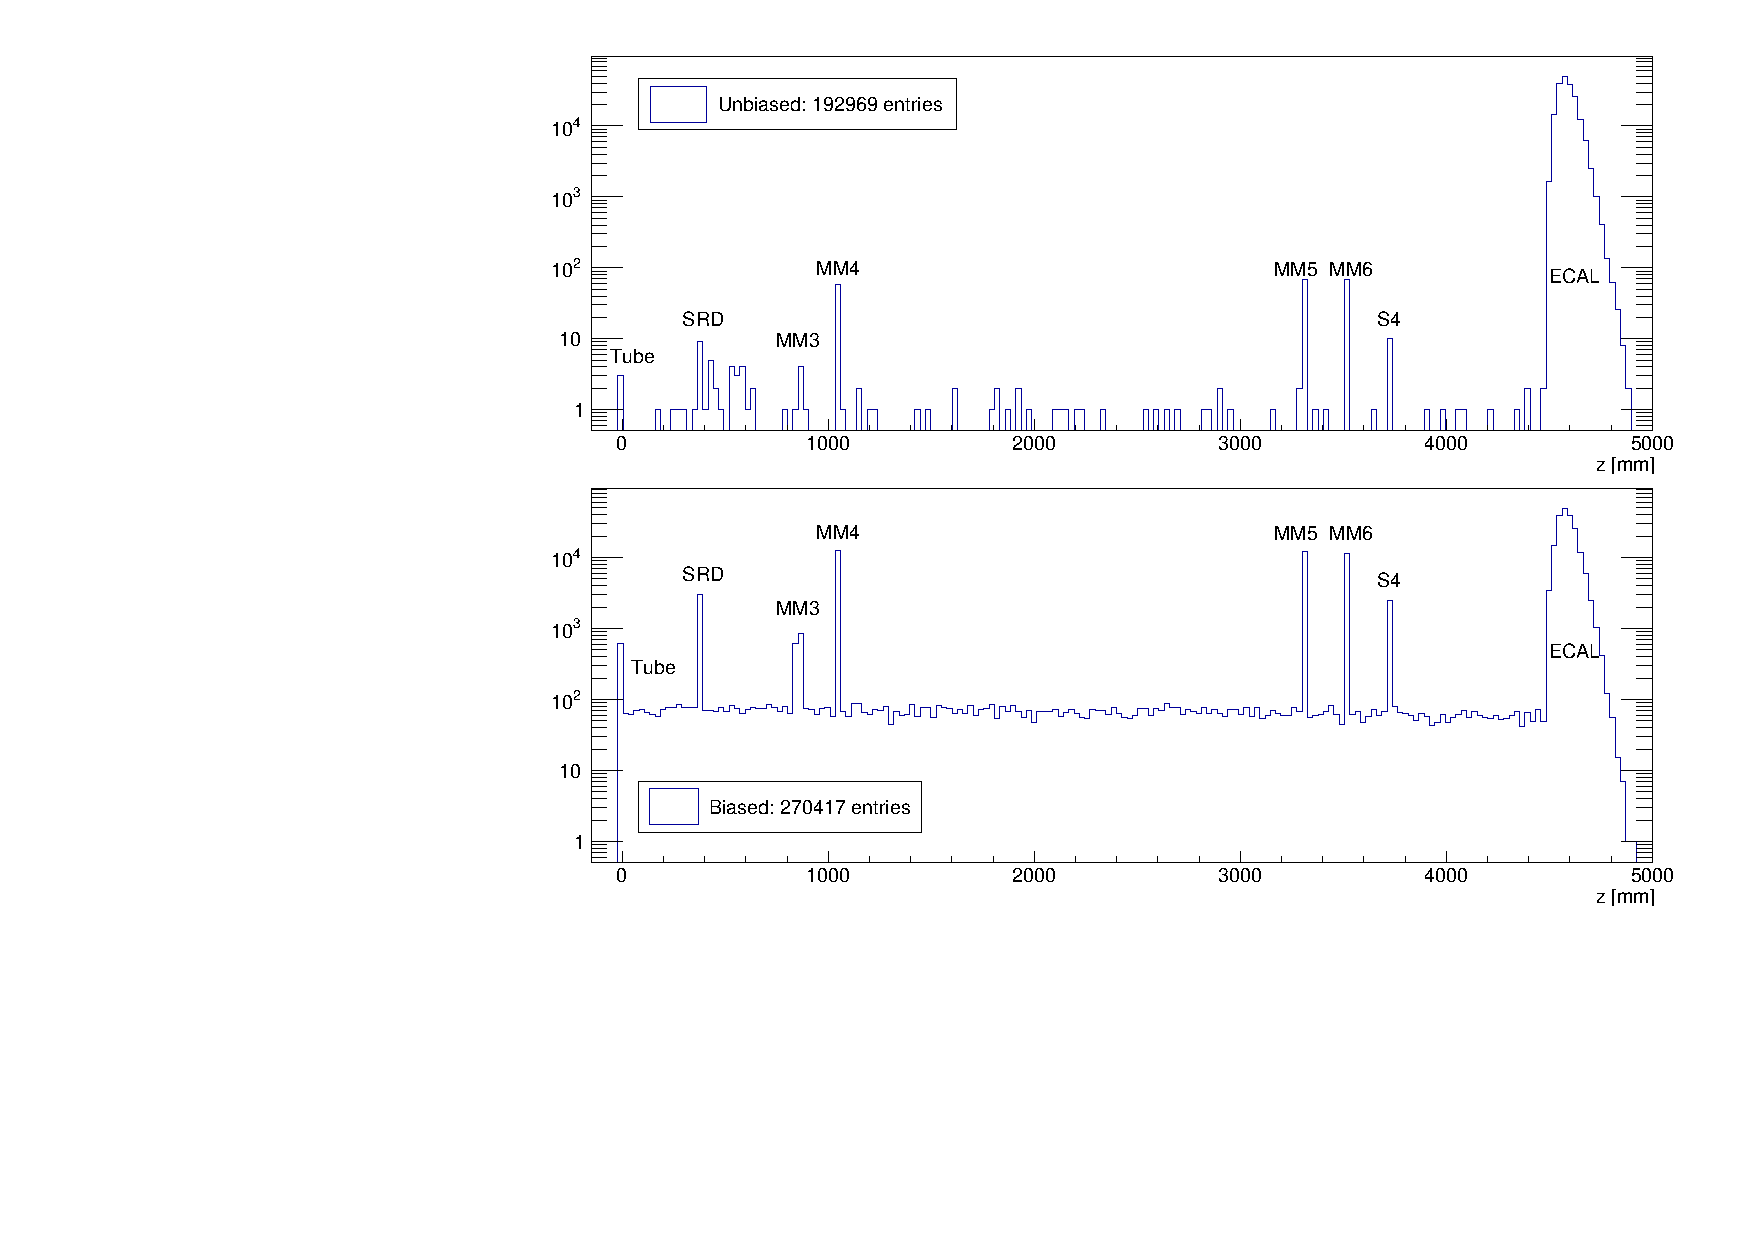
\includegraphics[width=0.9\linewidth]{\appdirc/pp70-enz-may3.pdf}
  \caption[Histograms of the z position of electronuclear interactions.]{Z position of electronuclear interactions between the end of the vacuum tube (0) and the ECAL (4500 mm) for biased ($k=200$) and unbiased simulations with $2.5\times10^6$~EOT each. No cuts applied. Note that MM3 has less dead material than the other MM detectors and thus is responsible for considerably fewer electronuclear interactions.}
  \label{res:fig:enz}
\end{figure}
%
which shows two histograms of the z position of electronuclear interactions between the end of the vacuum tube and the ECAL for biased and unbiased simulations. From this figure it can also be seen that the largest contribution to the upstream electronuclear interactions comes from the Micromegas detectors, with some additional contributions from the SRD and S4. Since the HCAL energy leak is proportional to the distance to the upstream interaction, we can conclude that MM4 constitutes the biggest source of hadronic background, with some additional contributions from MM3, the SRD and the vacuum tube window. \ref{res:Tab:biasgain} shows the increase (gain) of electronuclear interactions for the upstream detectors with and without the 80~GeV cut on the ECAL energy. The gains are in decent agreement with the biasing factor of 200.

\begin{table}[htbp]
	\centering
	\caption[Bias gain of upstream electronuclear interaction.]{Number of electronuclear interactions and bias gain for $2.5\times10^6$~EOT and a biasing factor of $k=200$.}
	\begin{tabular}{|c|c|c|c|c|c|c|}
		\toprule
		\multirow{2}{*}{\thead{\textbf{Detector}\\\textbf{Component}}} &\multicolumn{3}{c|}{\textbf{No cuts}}&\multicolumn{3}{c}{\textbf{E\textsubscript{ECAL} < 80 GeV}}\\
		\cmidrule(lr){2-7}
		& \textbf{Unbiased} & \textbf{Biased} & \textbf{Gain}& \textbf{Unbiased} & \textbf{Biased} & \textbf{Gain}\\
		\midrule
		Window & 3 & 615 & 205 & 0 & 27 & -\\
		SRD & 10 & 3079 & 308 & 1 & 117 & 117\\
		MM3 & 5 & 1472 & 294 & 0 & 56 & -\\
		MM4 & 58 & 12714 & 219 & 4 & 514 & 129\\
		MM5 & 70 & 12145 & 173 & 4 & 549 & 137\\
		MM6 & 69 & 11279 & 163 & 2 & 425 & 212\\
		S4 & 10 & 2473 & 247 & 0 & 77 & -\\
		ECAL & 192219 & 191637 & 1 & 36 & 216 & 6\\
		\bottomrule
	\end{tabular}
	\label{res:Tab:biasgain}
      \end{table}

\begin{table}[htbp]
	\centering
	\caption[MC cut efficiencies for the simulation with bias $k=200$ and $1.79\times10^7$ EOT.]{MC cut efficiencies for the simulation with bias $k=200$ and $1.79\times10^7$ EOT. Listed are the fraction of surviving events. The individual efficiencies are calculated relative to the the 80~GeV cut. The cumulative efficiencies are calculated relative to the EOT. Cumulative efficiencies below the horizontal line are calculated relative to the cumulative efficiency of the cuts above the line.}
	\begin{tabular}{|cccc|}
		\toprule
		\textbf{Cut} & \thead{\textbf{Surviving}\\\textbf{Events}} & \thead{\textbf{Efficiency}}& \thead{\textbf{Cumulative}\\\textbf{Efficiency}}\\
		\midrule
		Trigger & 1.48$\times10^{7}$ & - & 0.83\\ 
		80~GeV cut & 22'305 & 1 & 1.3$\times 10^{-3}$\\
		SRD cut & 19'500 & 8.7$\times 10^{-2}$ & 1.1$\times 10^{-3}$\\
		$\chi^2$ cut & 3069 & 2.1$\times 10^{-2}$ & 1.7$\times 10^{-4}$\\
		ECAL center & 3022 & 8.6$\times 10^{-2}$ & 1.7$\times 10^{-4}$\\
		Zero degree HCAL & 2938 & 9.6$\times 10^{-2}$ & 1.6$\times 10^{-4}$\\
		Dimuon cut & 2615 & 9.8$\times 10^{-2}$ & 1.5$\times 10^{-4}$\\
		\midrule
		ST 123 & 2214 & 8.2$\times 10^{-2}$ & 1.2$\times 10^{-4}$\\
		VETO & 1755 & 7.9$\times 10^{-2}$ & 9.8$\times 10^{-5}$\\
		ST 12|23 & 1485 & 6.7$\times 10^{-2}$ & 9.8$\times 10^{-5}$\\
		ST 1|2|3 & 481 & 2.2$\times 10^{-2}$ & 2.7$\times 10^{-5}$\\
		\bottomrule
	\end{tabular}
	\label{res:Tab:mccuts}
      \end{table}

\section{Modification of the Fritiof String Model}
\label{appC:sec:ftfp-modifications}

In this section we provide a specific example of how the simulation is corrected using data from the calibration runs that was part of my work. In this instance we improve the energy deposited inside a calorimeter in events with intranuclear inelastic scattering. A large amount of events where an incoming hadron deposit all its energy inside an electromagnetic calorimeter was observed in the simulation and not reproduced in the data.
% The reason of this deviation might be that most of hadronic models are optimized for a scenario where $\lambda_{int}$ of the target is large enough to stop completely the incoming hadron on average, which is not the case for the ECAL or the WCAL. As large em-shower triggered by hadrons is a source of background in the visible mode, this comparison is particularly significant to estimate the background of this mode precisely.

We compare the data and predictions by simulating a sample of $\pi^-$ and compare the distribution with the data of an hadron calibration run and do the same for $e^-$. The result of this first comparison is shown in Fig.\ref{fig:ecal-comp}. In the first plot, we see the energy deposited in the WCAL for electrons measured in the calibration run compared to what is predicted by our MC. As expected because of the QED nature of the process, the two distributions agree quite well in the core, with some minor disagreement in the tail mostly due to pileup. On the other hand, even after accounting for the detector corrections, we can see that there is a fundamental disagreement at the end of the spectrum when the comparison is performed with pions, specifically in the region relevant for deep inelastic scattering. Since the disagreement is large when all the nominal energy of the beam is deposited inside the target, the disagreement appears to be caused by some electron contamination in the hadron beam. However, the data were filtered by requiring less than 1 MeV energy deposited in each SRD counter facing the beam inlet. This reduces the contamination conservatively at a level $<$0.01\%, which is far below the disagreement observed. A faulty calibration is also unrealistic since the agreement with electrons is excellent in that energy range. The simulation systematically overestimates the number of events in the region where most of the energy released in the inelastic scattering is emitted in the form of $\pi^0$,$\eta$, $\eta'$ which trigger an em-shower completely contained in the calorimeter.

\begin{figure}[bth!]
  \centering
  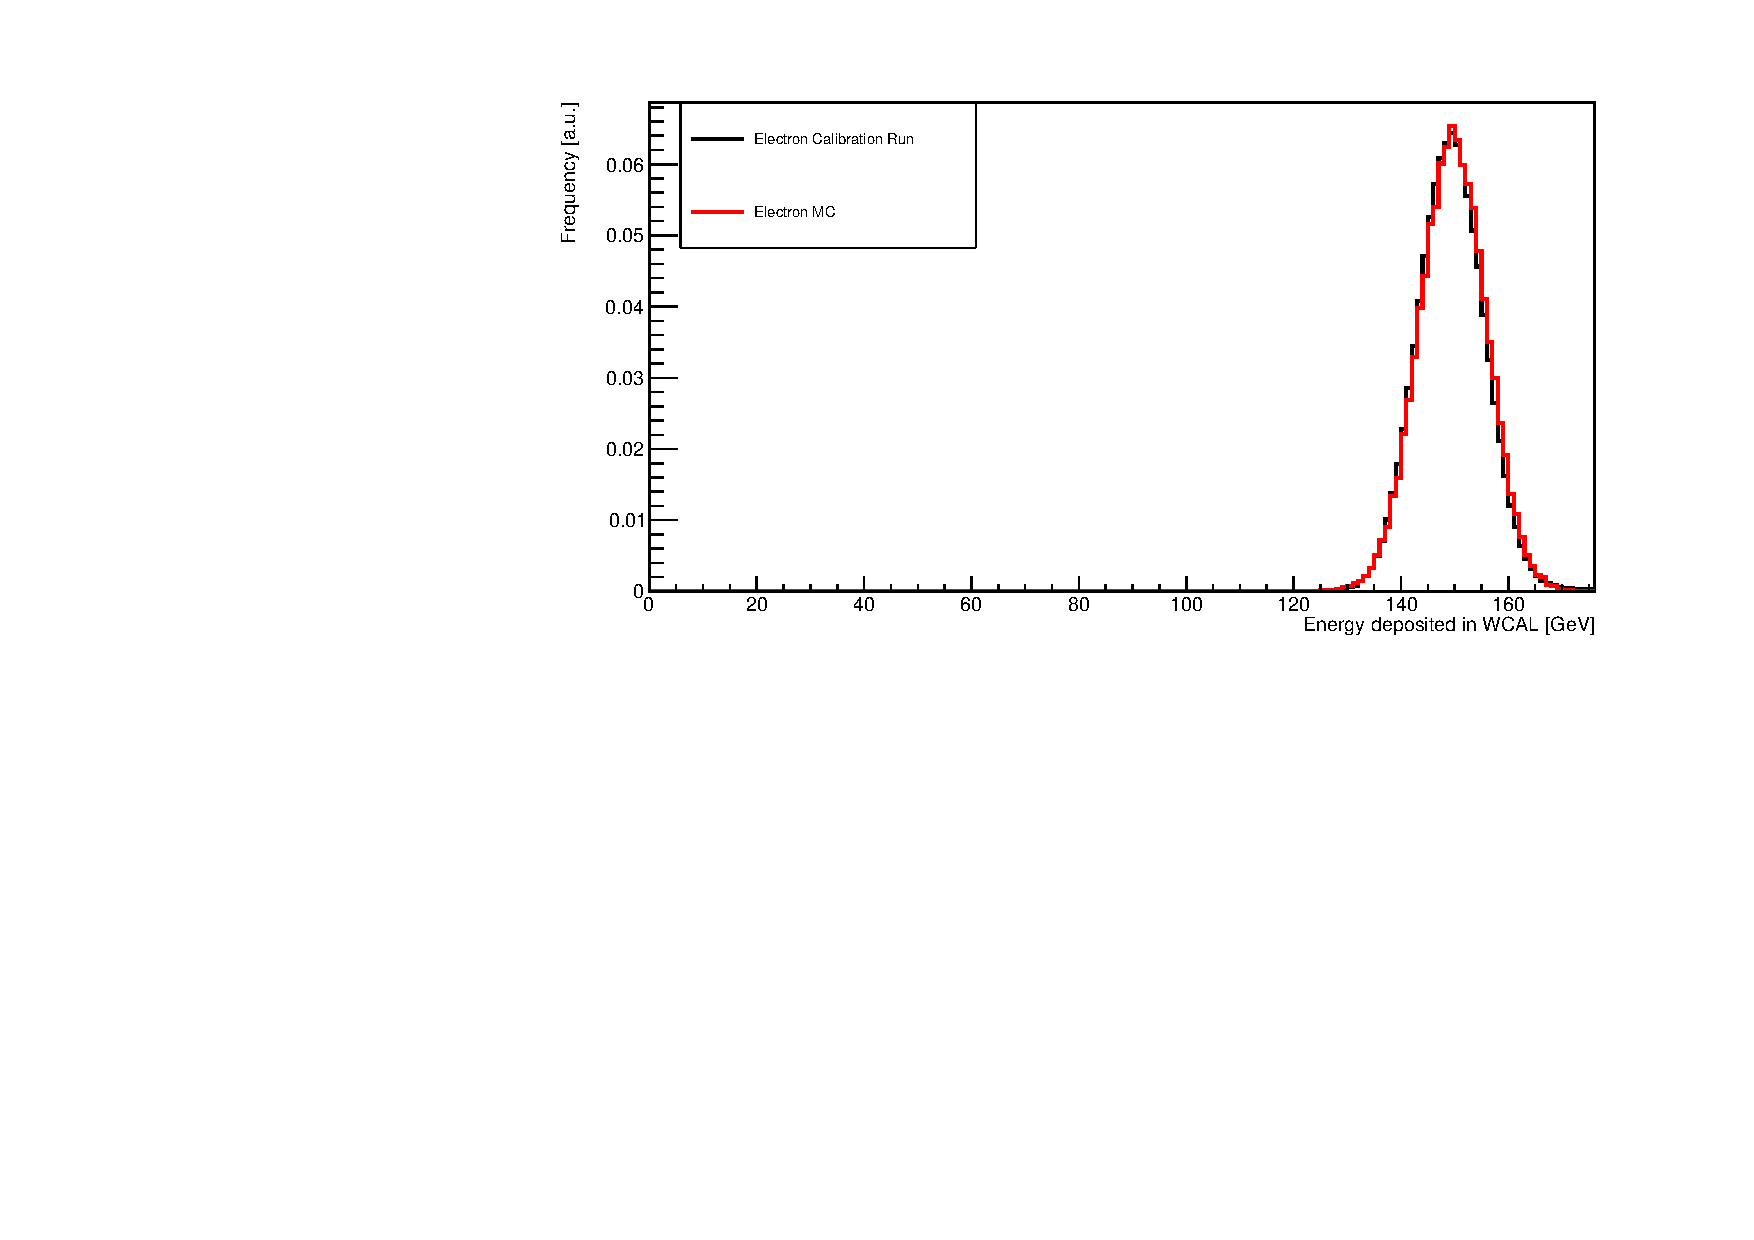
\includegraphics[scale=0.6]{\appdirc/wcal_elec_comp.pdf}
  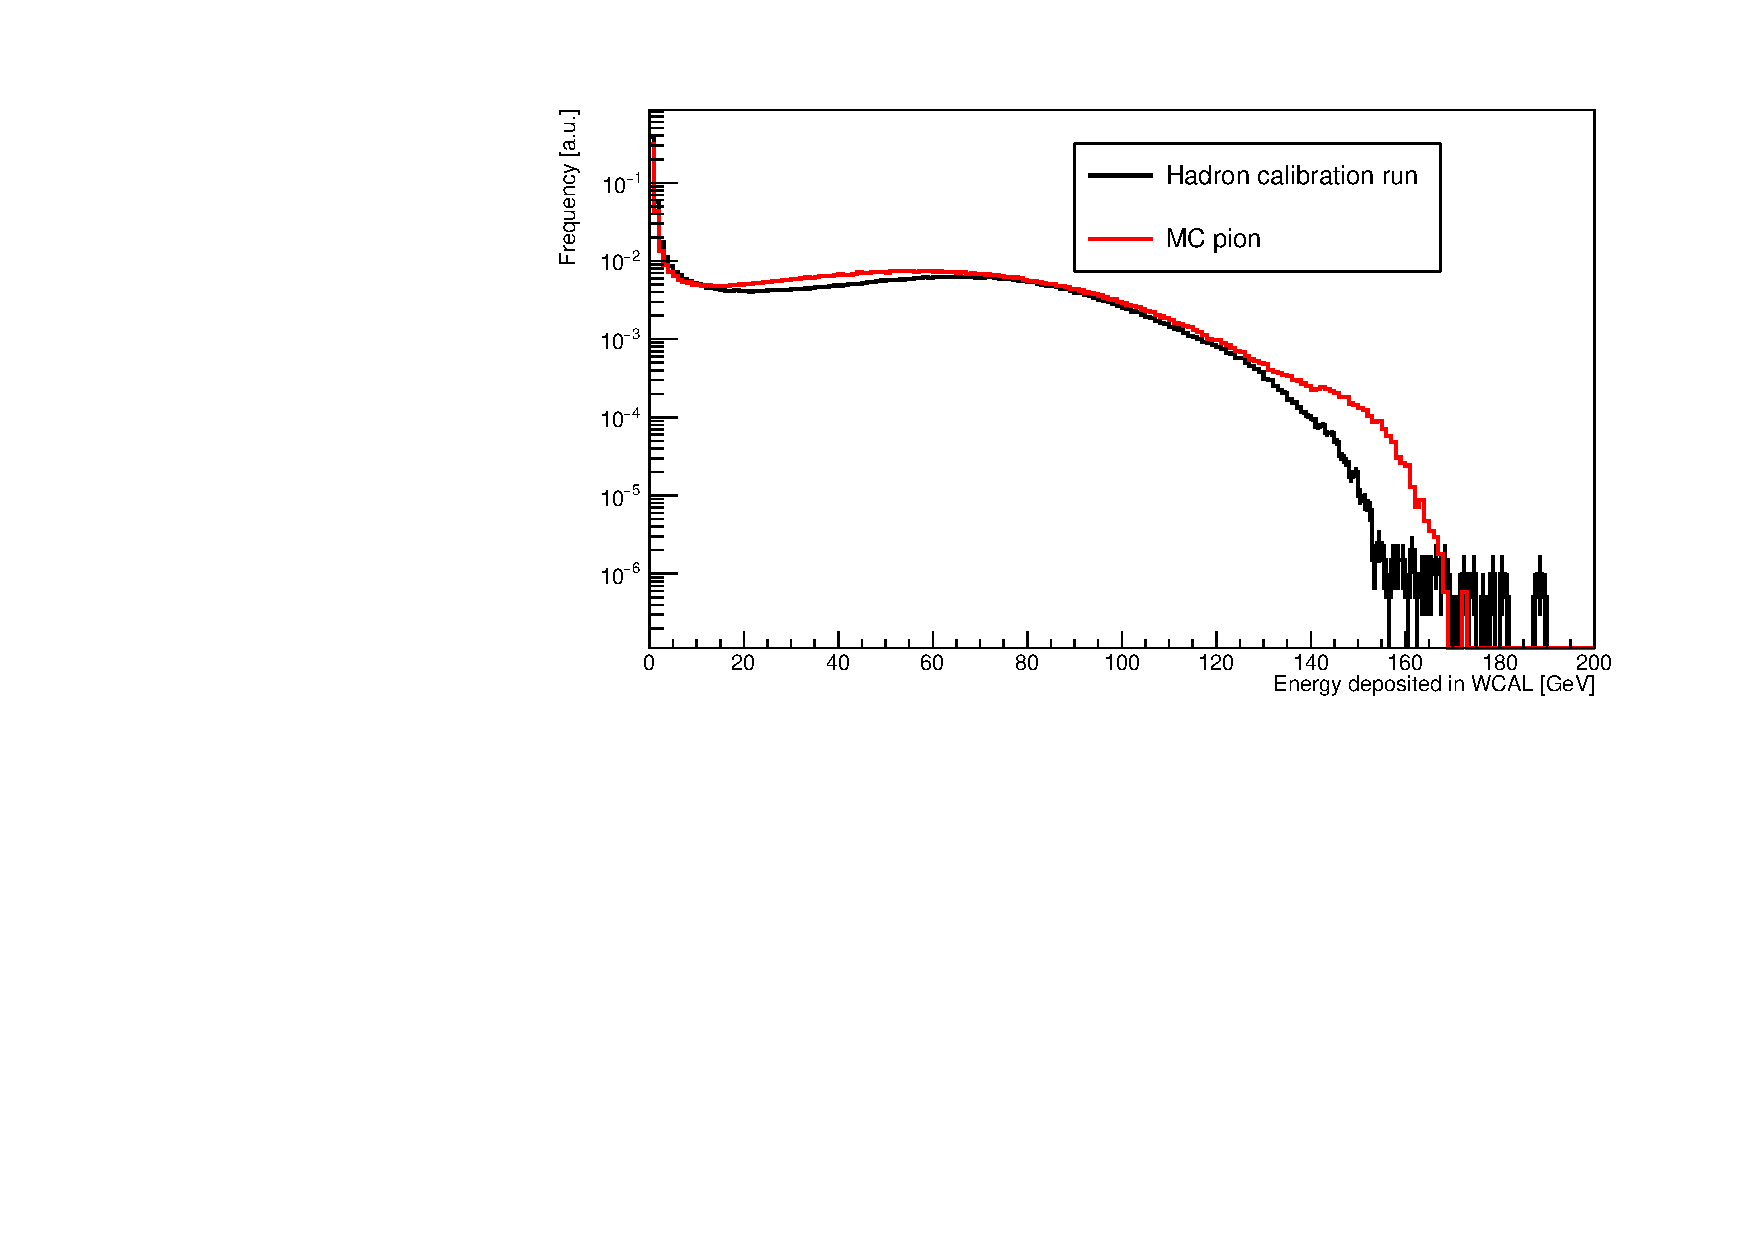
\includegraphics[scale=0.6]{\appdirc/wcal_pion_comp.pdf}
  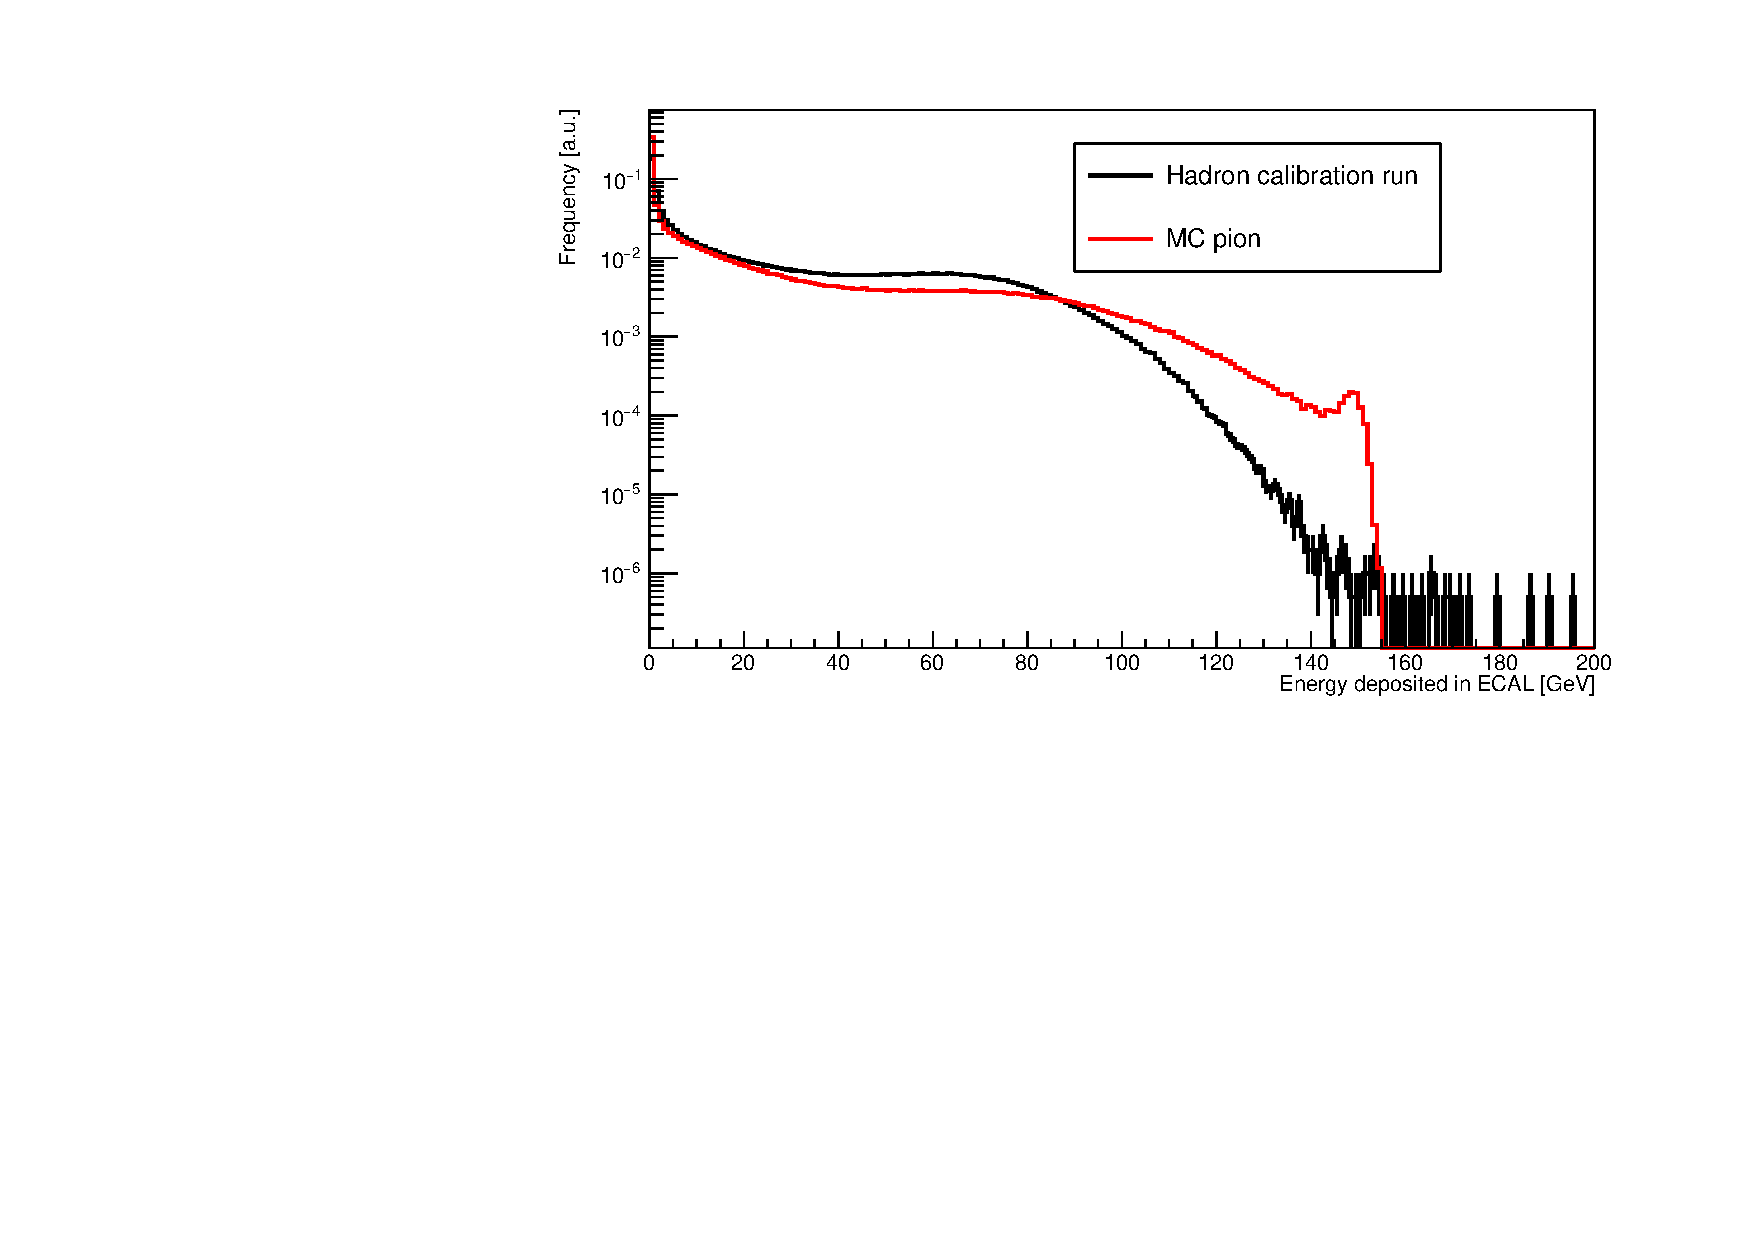
\includegraphics[scale=0.6]{\appdirc/ecal_pion_comp.pdf}
  \caption[MC/DATA Comparison of $\pi^-$ in ECAL and WCAL]{Comparison between MC and data for different detectors and different runs. Top: WCAL energy deposited for electrons, Middle: WCAL energy deposited for hadrons, Bottom: ECAL energy deposited for hadrons.}
  \label{fig:ecal-comp}
\end{figure}

To investigate this mismatch, a complete comparison between different physics lists was performed to investigate 
different models. We used the energy deposited in the WCAL as a benchmark for this comparison, and simulate the interaction of $\pi^-$ using two alternative physics list. The \textit{QGSP\_FTFP\_BERT}, which uses the alternative Quark-Gluon String model to simulate hadrons at energy higher than 25 \gev, and the \textit{FTFP\_BERT\_TRV}, which uses the recommended Fritiof model but with an alternative method for the elastic scattering \cite{AGOSTINELLI2003250}. The result is shown in Fig.\ref{fig:geant4-hadron-plist}, the recommended physics list has the best agreement for high energy deposit, but for all three the disagreement remains significant. The QGSP model, although offers the worst prediction at high energy, has better agreement after in the range 25-80 $\gev$.

\begin{figure}[tbh!]
  \centering
  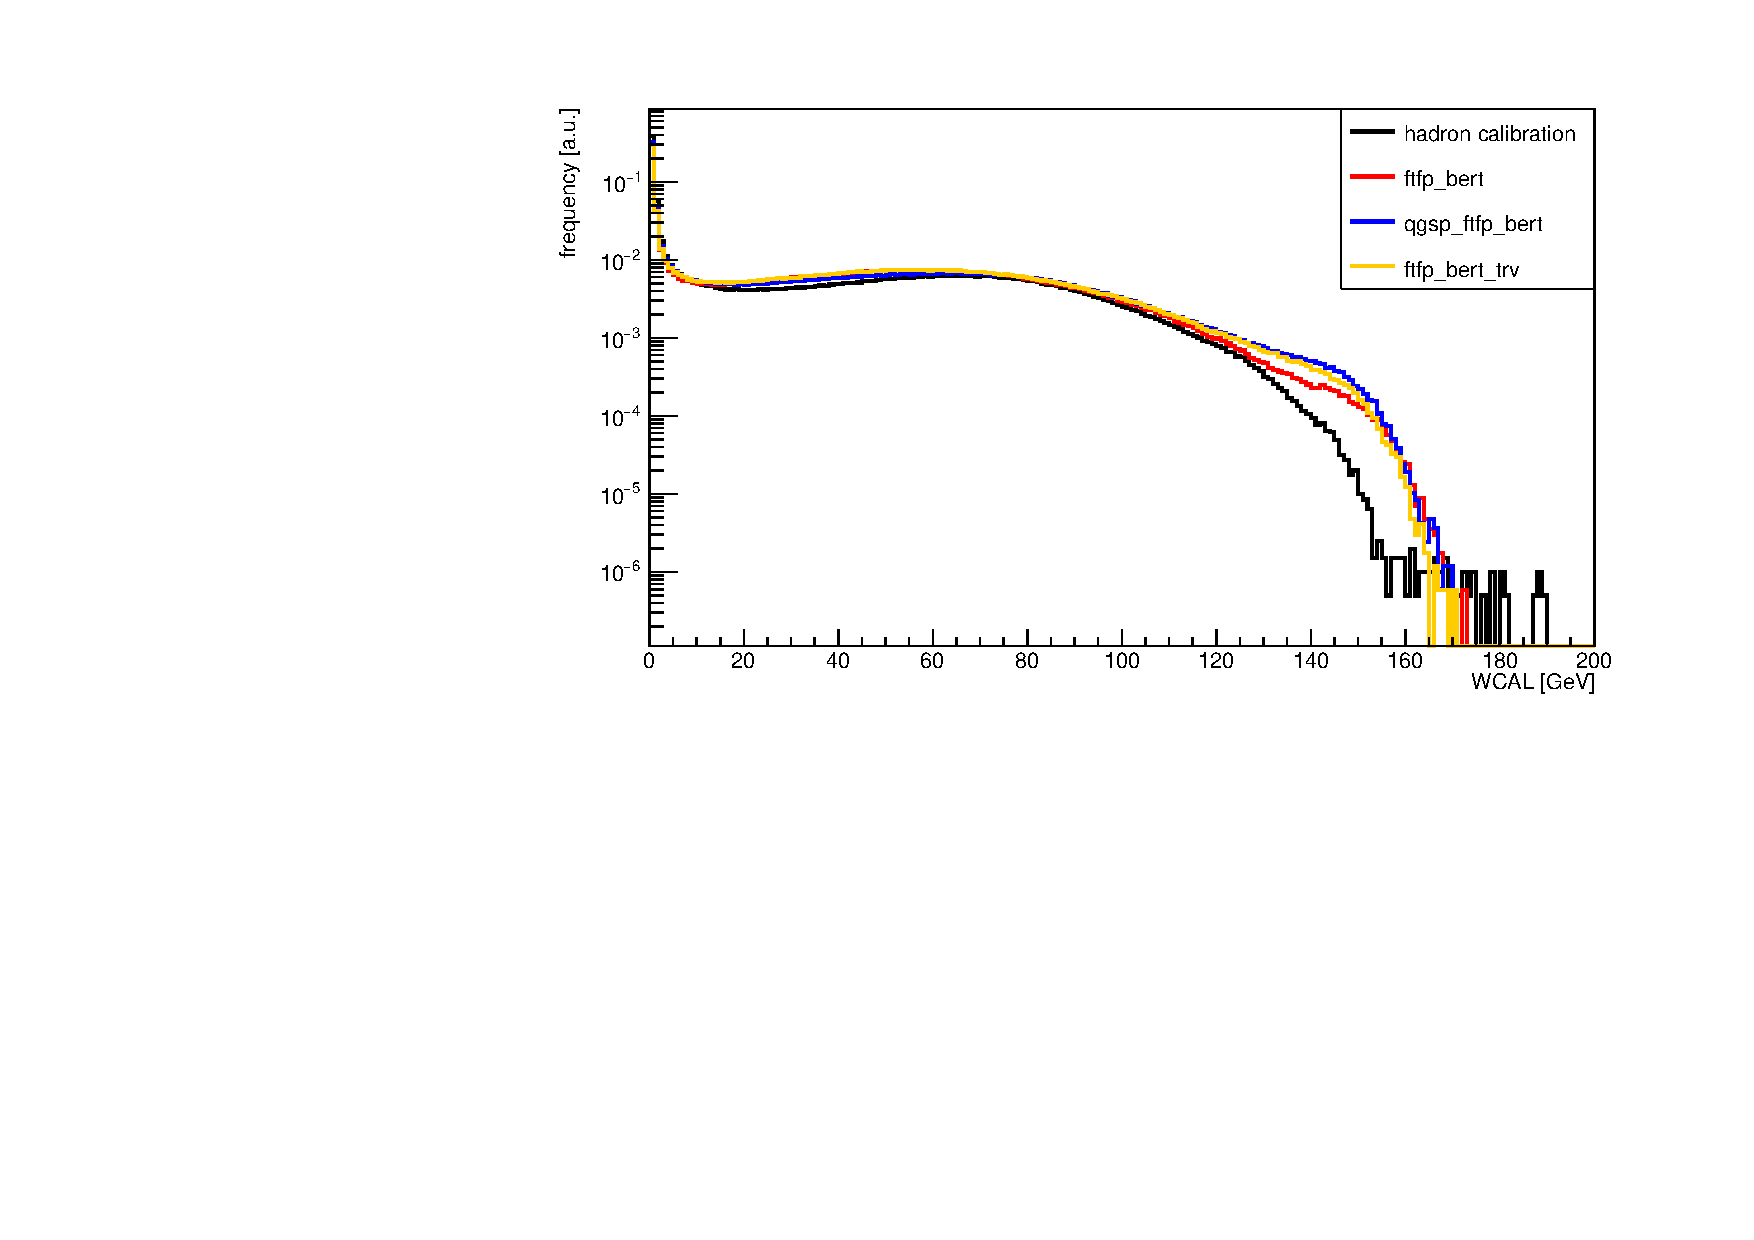
\includegraphics[width=\textwidth]{\appdirc/physlist_v1.pdf}
  \caption[Comparison of physics list for $\pi^-$ in WCAL energy spectrum]{Energy deposited in WCAL for different physics lists. Data collected in the hadron calibration run in 2018 are plotted in black.}
  \label{fig:geant4-hadron-plist}
\end{figure}

The next test performed was to simulate different particles in the setup. The three main contributions to the beam impurities in H4 were simulated using the \textit{FTFP\_BERT} physics list: $\pi^-$, K$^-$, and p$^-$. Here a significant improvement is visible in the case of anti-proton (Fig.\ref{fig:geant4-hadron-particles}), where data and MC are compatible at the tail of the distribution. This would suggest that such an event is caused by charge-exchange interaction between pions and the target nucleus, enhanced for light mesons. To date, no proper treatment is offered by Geant4 for this process, which means the disagreement must be caused by an improper treatment of hadronization in the limit of diffraction,  where most of the energy is exchanged between two partons: one of the nucleus and one of the projectile impacting it. The discussion becomes here more complicated and requires the tuning of specific parameters inside the FTF model.  The \textit{FTFP\_BERT} physics list was modified as illustrated in Appendix \ref{appC:sec:ftfp-modifications} to experiment with different possibilities. The target diffraction and the projectile diffraction were switched on and off respectively to investigate the effect on the distribution.


\begin{figure}[tbh!]
  \centering
  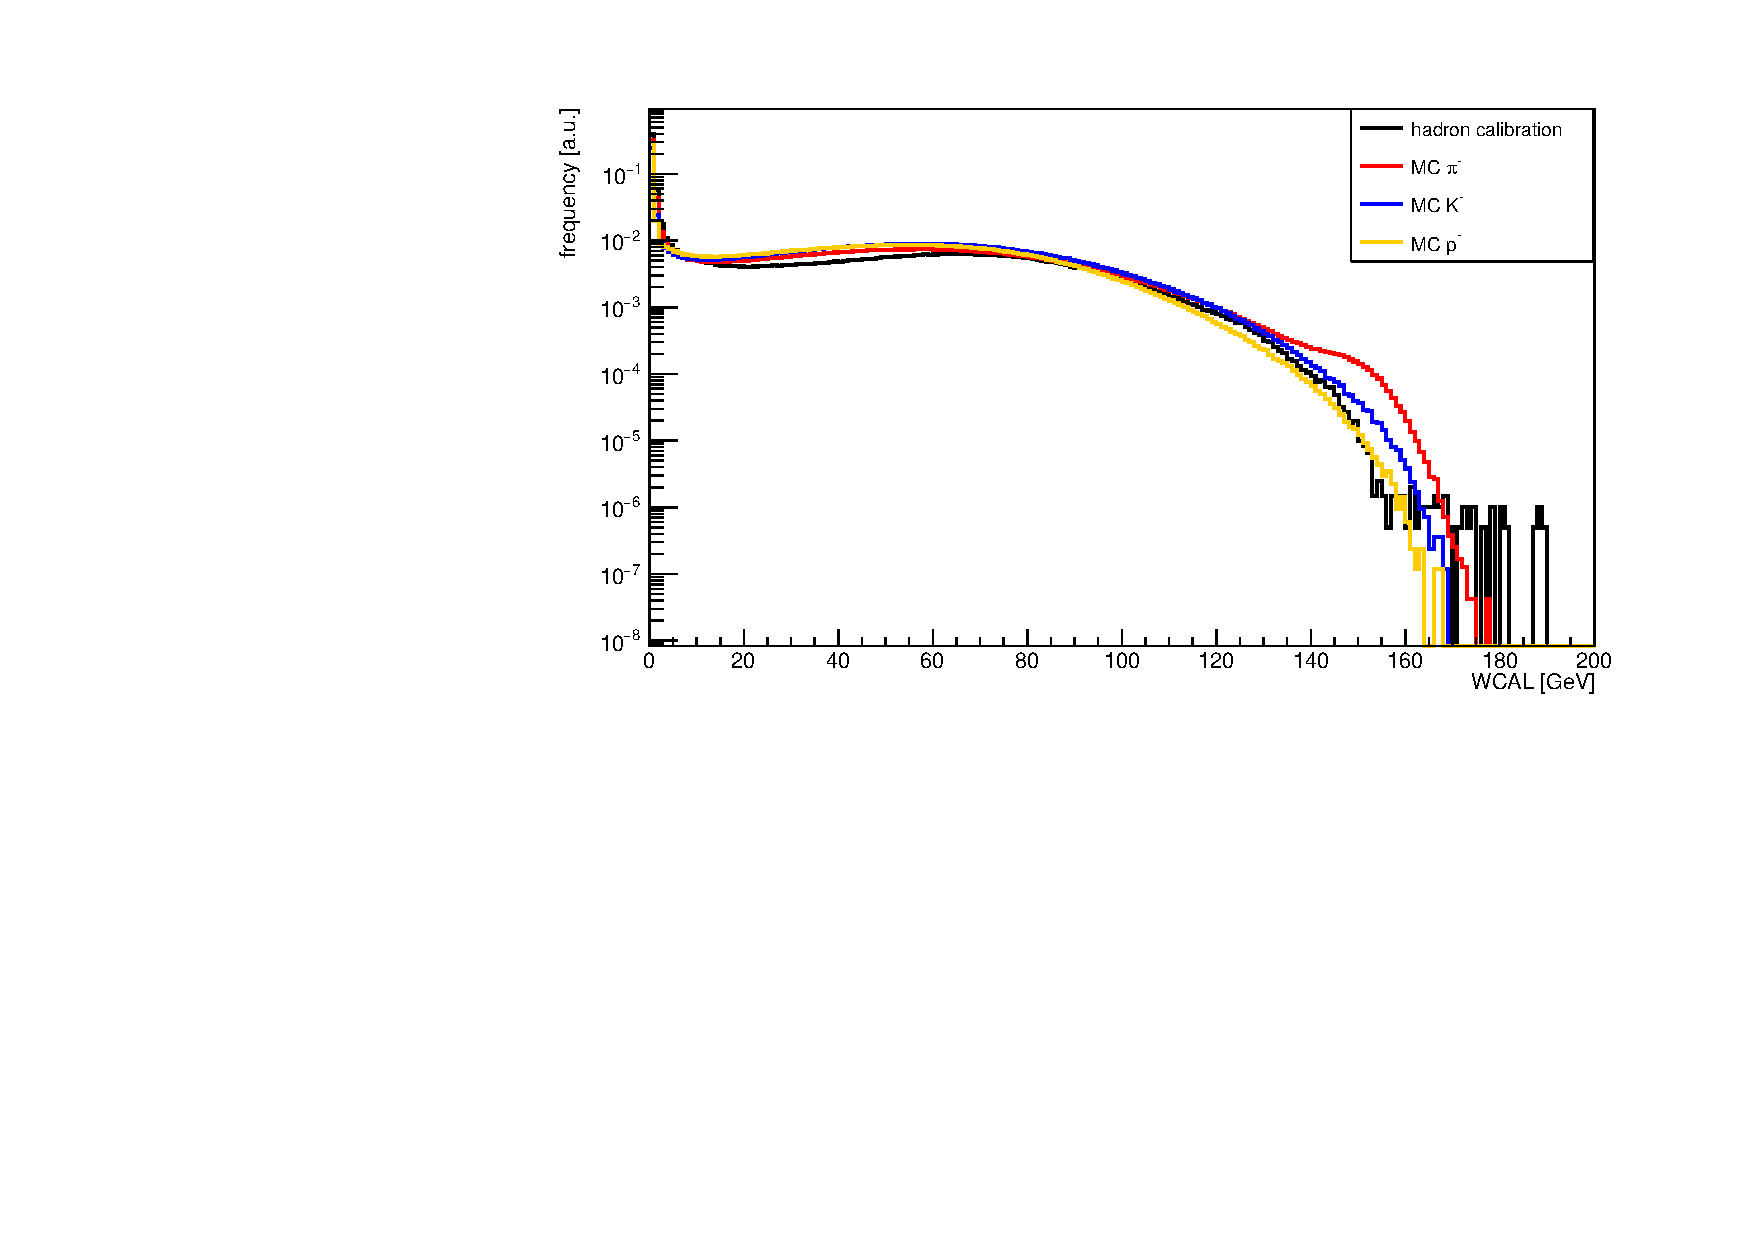
\includegraphics[width=\textwidth]{\appdirc/physlist_particles.pdf}
  \caption[Comparison of different simulated hadrons in WCAL energy spectrum]{Comparison of different simulated hadrons in WCAL energy deposit.}
  \label{fig:geant4-hadron-particles}
\end{figure}

\begin{figure}[tbh!]
  \centering
  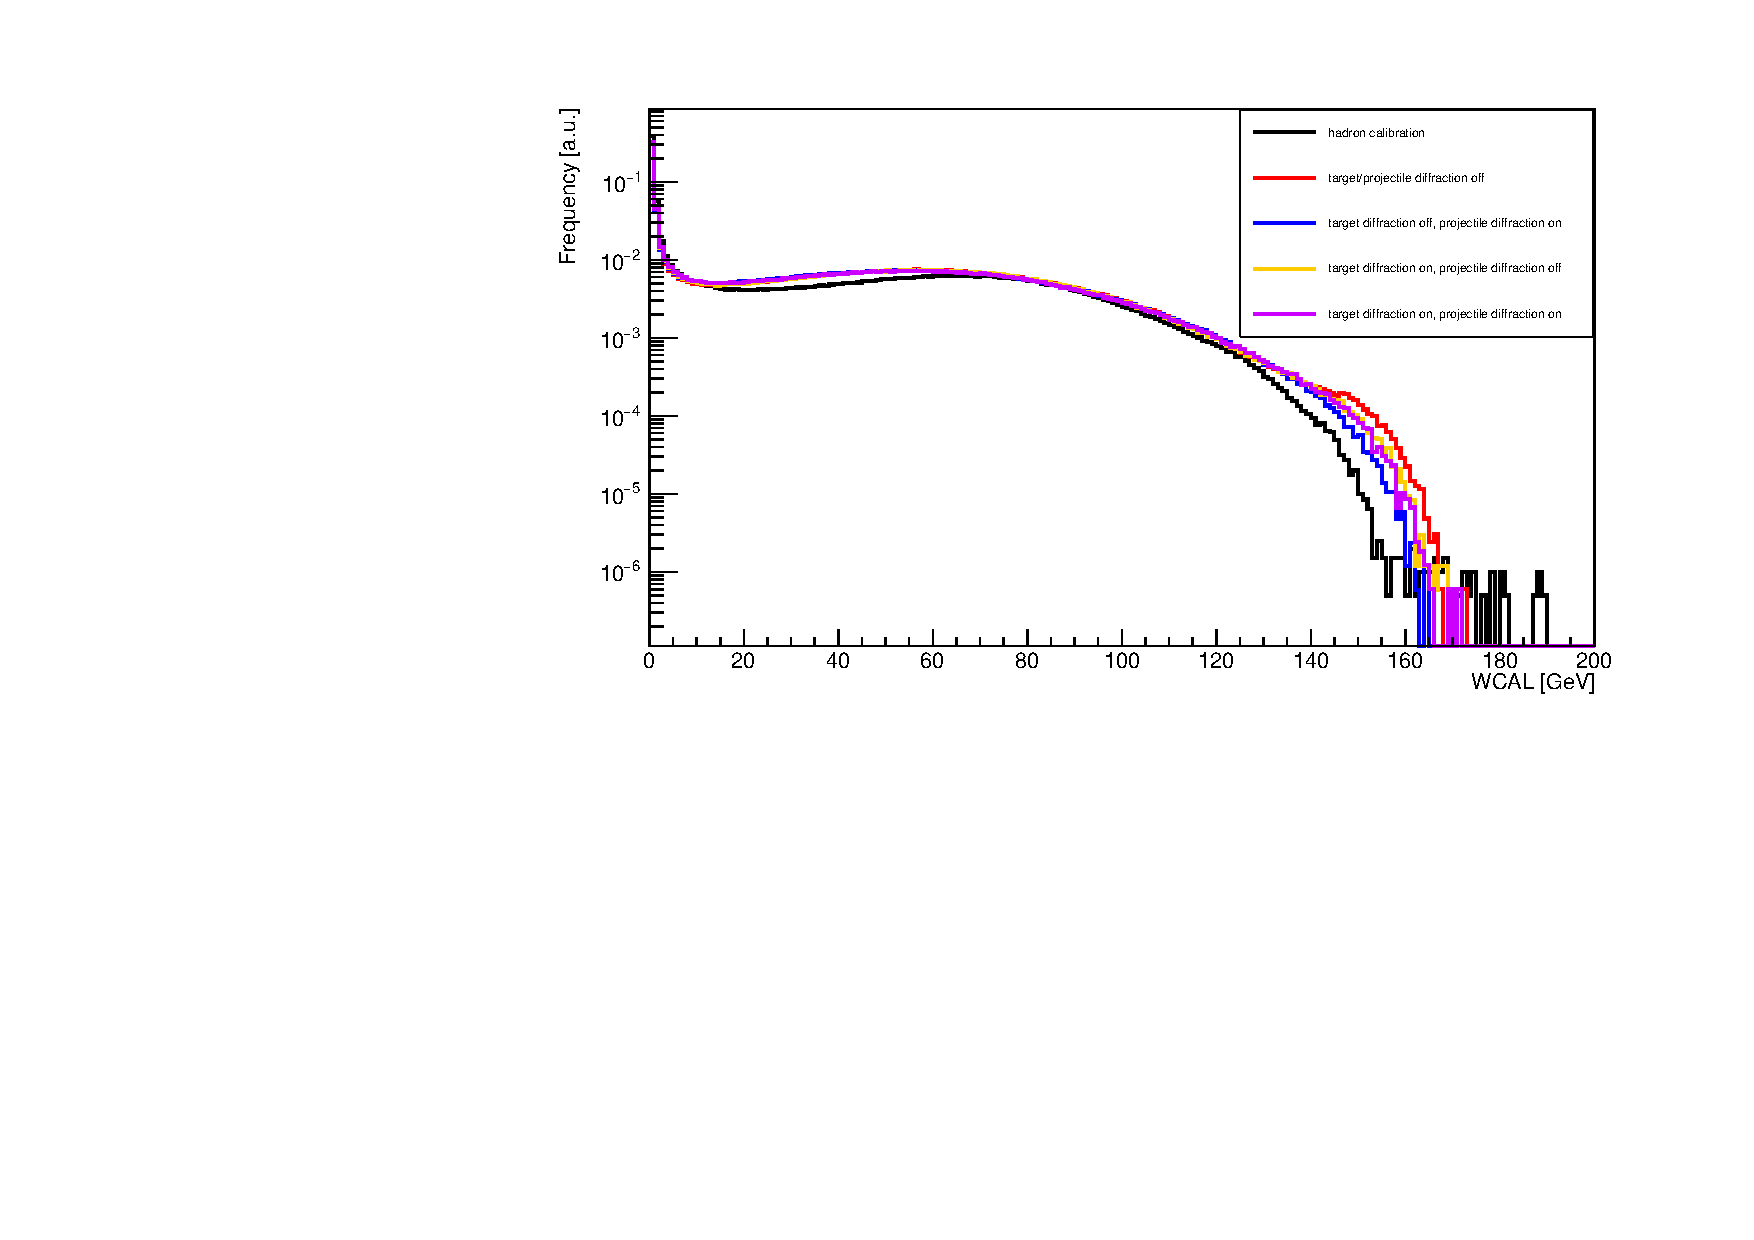
\includegraphics[width=\textwidth]{\appdirc/physlist_diffraction.pdf}
  \caption[Comparison of different diffraction limits for hadrons in WCAL energy spectrum]{Comparison of simulated $\pi^-$ in WCAL energy deposit using the physics list $FTFP\_BERT$ using different parameters for the model. Main difference between models is the diffraction of target or projectile, which is switched on and off.}
  \label{fig:geant4-hadron-diff}
\end{figure}

The conclusion of this comparison (Fig.\ref{fig:geant4-hadron-diff}) is that the largest contribution to the disagreement comes from the projectile diffraction incorrectly excluded in the standard \textit{FTFP\_BERT} physics list, whereas target diffraction contributes instead negatively to the residual.

Some modifications of the \textit{FTFP\_BERT} were decided to improve the agreement in the distributions considered. The target diffraction was switched off, the projectile diffraction was switched on, and the parameters of the FTF model were modified to shift the behavior of $\pi^-$ to the one predicted for an anti-baryon. This is performed by acting mostly on the probability of each quark to be involved in the scattering and the average energy exchanged between partons. The final result is shown in Fig.\ref{fig:geant4-hadron-final}, the disagreement for the high-energy spectrum improves, with some overestimation of the probability of large inelastic scattering still present in the energy range 25-80 \gev. The disagreement for deposit larger than 20 $\gev$ is now $\sim$15\%, improved by a factor 2 compared to the original model.

\begin{figure}[tbh!]
  \centering
  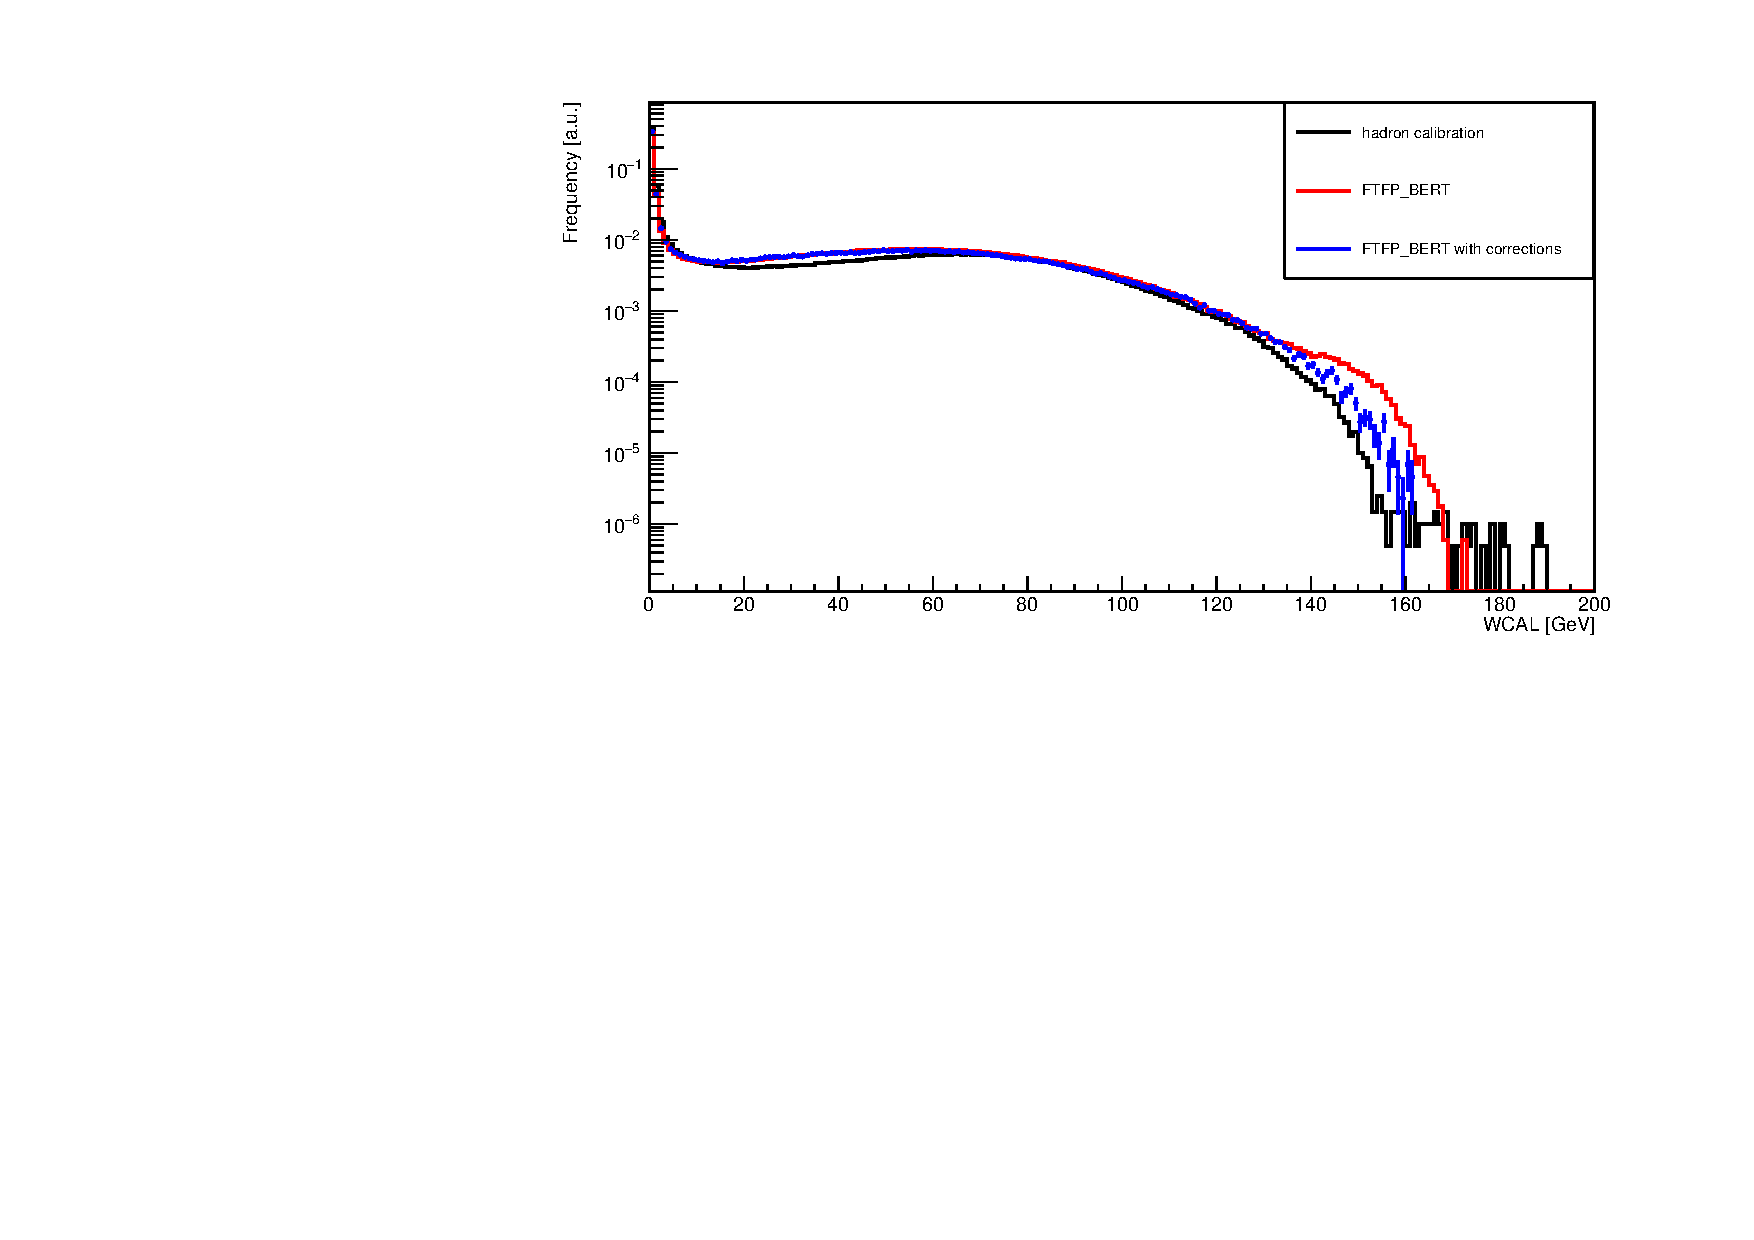
\includegraphics[width=\textwidth]{\appdirc/final_comp.pdf}
  \caption[Comparison of hadron energy deposit after corrections]{Comparison between data (black line) and simulated $\pi^-$ in WCAL energy deposit using the physics list $FTFP\_BERT$ before and after corrections applied to the model.}
  \label{fig:geant4-hadron-final}
\end{figure}

%%% Local Variables:
%%% mode: latex
%%% TeX-master: "../PhDthesis"
%%% End:
